\documentclass[12pt]{report}
\usepackage{titling}
\usepackage{geometry}
\usepackage{graphicx}
\usepackage{listings}
\usepackage{color}

\definecolor{dkgreen}{rgb}{0,0.6,0}
\definecolor{gray}{rgb}{0.5,0.5,0.5}
\definecolor{mauve}{rgb}{0.58,0,0.82}

\lstset{frame=tb,
  language=Java,
  aboveskip=3mm,
  belowskip=3mm,
  showstringspaces=false,
  columns=flexible,
  basicstyle={\small\ttfamily},
  numbers=none,
  numberstyle=\tiny\color{gray},
  keywordstyle=\color{blue},
  commentstyle=\color{dkgreen},
  stringstyle=\color{mauve},
  breaklines=true,
  breakatwhitespace=true,
  tabsize=3
}

\geometry{margin=1in}
\begin{document}
\title{Final Documentation for 32 Pounds\\ \vspace{2 mm} {\large CS 383: Software Engineering}}

\author{32 Pounds}
\date{\today}
\maketitle
\clearpage
\tableofcontents

\begin{chapter}{Project History}
	
	Initially our project design was based primarily on working to fulfill homework requirements and trying to keep everything scrum based.  
	For our group most of scrum work was new, really implementing project design was something most of us haven't done.  
	Our typical work load was code, code, and more code.  At the beginning this seemed to be a setback for our team, we had trouble focusing on setting up requirements, use cases, and class diagrams instead of just jumping straight into code.  
	The workload wasn't necessary unbearable or hard, it was just a different process than most of us were used to.  
	As a team we thought that it would have been easier to code and then set up these diagrams based on our code, but when setting up a business idea you must have an actual plan before you have the code, so this was essential.  
	
	Lets move to project design.
	We had high hopes for our game which was acceptable but later in the semester was not very feasible.  
	This was ok because this class isn't necessarily based on the project outcome but really learning to work by the scrum techniques and to incorporate software design principles. 
	We were about half way through the semester with very little coding done, design was in place but we were waiting on implementing anything due to the lack of knowledge of what the next homework was going to be. 
	Basically half way through the semester we had nothing but design and a main menu. 
	Previous students who took CS383 warned us of choosing a game because it seemed to be more difficult than expected.  
	Most likely because expectations are high when it comes to games and experience in making them is somewhat low.  
	For our group our experience varied, we have a couple very good programmers and others that aren't as efficient.  
	Java wasn't necessarily a “first” language for most of us so having to learn java and work on a fairly difficult project was somewhat tough.  
	As a team we diverted, some worked primarily on code while others worked on map, sprite art, documentation, and other necessary tasks.  
	
	Lack of time and experience seemed to hinder us from the initial game design we had developed.  
	This was expected, we had to adapt and pick what we deemed to be most important from our backlog.  
	This is where we chose to diverge from a very developed storyline and work more into networking.  
	Networking was something our team wasn't very confident with so we decided it would be beneficial for us to work on that rather than playing with player and quests and such.
	
	We decided to keep our initial documentation and also to make current documentation to see how things varied throughout the semester.  
	Here are the designs that changed the most throughout the semester.
	
	\begin{enumerate}
		\item Player design
		\item Advanced gameplay i.e quests, factions, inventory
		\item Multiplayer
	\end{enumerate}
	
	\begin{subsection}{Player Expectations}
		Initially we had a couple of different ideas drawn out for our main player character.  
		We wanted a player inventory, player skills, and a faction or group that the player could join.  
		We decided to that this would mean that we would need to incorporate a very defined story line that was single player heavy, 
		which we did not want to do. The ideas for the player were scrapped do to the fact that we would rather create a better 
		multiplayer environment than a single player environment.
	\end{subsection}
	
	\begin{subsection}{Advanced Gameplay}
		Gameplay is something where the idea seems so easy but the implementation 
		takes much more thought.  So much needed to be implemented before we started gameplay 
		that we never really got around to it.  For instance, our game was structured for single player 
		until we decided to reroute to multiplayer.  The gameplay was different for a single 
		player than it is for multiplayer in our game.  Before we can completely work on the 
		gameplay we wanted i.e quests, combat, factions, we needed inventory, player health, moving monsters,
		and also monsters that react to your movement which is more difficult than one would think. 
		We ended up with making a gameplay in which you run around killing bugs that have invaded your office
		space, some bugs attack you, others dont. 
	\end{subsection}
	
	\begin{subsection}{Multiplayer}
		Much of the final sprint was dedicated to Multiplayer. It became a project fork around 
		homework 6.  The decision to focus on multiplayer was motivated by three key reasons: We had spent
		considerable effort keeping the code base compatible with a multiplayer mode, Many of us were interested
		in the experience of making a multiplayer game, and we though that we might be the only team to successfully acheive full multiplayer.  We set up a meeting where the details of multiplayer were hashed out, like the structure of our packets.  We chose to send the complete state of the game through a UDP packet at 40 packets
		per second so that the same packet would apply to all clients, and we don't have to remember which entities have moved.
	\end{subsection}
\end{chapter}



\begin{chapter}{Implementation details} 
 Our game can be run with ``gradle run" from the ``OSGame" directory within our project, or by running the jar file in the top level of our github repository. Both the client and the server are run from the same code, in fact every instance of the game is running a server and a client locally. The game has been tested to work freely within and between Windows, OS X, and Ubuntu and Arch Linux, although there are known issues when running in openJDK 7.
 
 To run our game, simply launch the jar file. Network communications use UDP ports 5050 and 5051. To join a game, press ESC, then ``join game", and then enter the IP address of a computer running another instance of the game. The other instance only needs to be running, it is not necessary for them to press "Host Game" or to even be playing in their local game at the time.
 
 Gradle has been used to manage almost every aspect of the build process. Many team members have used its good, if limited, support for netbeans and eclipse to build from within their IDE.
 
 The code is organized first between the ``core" and the ``desktop" folder. ``core" contains the platform independent code, which is the vast majority of our code base. ``desktop" contains a main class that deals with the specific considerations of launching our game on a desktop computing environment. If we wished to expand to other platforms, only the code within the desktop folder would need rewritten within a new folder. 
 
 Inside of ``core/src" exists most of our game's source code, split between the ``com" with the application code and ``test" with our unit tests. Within ``com" and ``test" are corresponding sets of .java files in a number of different subsystem directories.
 
\end{chapter}


\chapter{Initial Project Design: Use Cases}
This chapter presents the initial use cases based off the major systems in the game. These categories
include the player, monster, communications, game state and map.
  
  \begin{section}{Player Use Cases}
    \begin{subsection}{Speak with NPC}
      \textbf{Goal}:
      Player wishes to speak with an NPC in order to gain information or recieve 
      a quest.
      
      \textbf{Actors}:
      Player, NPC

      \textbf{Preconditions}:
      \begin{enumerate}
        \item The player is adjacent to an NPC.
        \item The NPC has an available speak interact command
      \end{enumerate}

      \textbf{Summary}:
      The player communicates with an NPC that is occupying the nearby space 
      in the world. Communication will add new game information and/or start
      a new quest.

      \textbf{Related Use Cases}:
      This use case extends the Interact with Coworker use case, and will be 
      connected to use cases coorelating to interacting with NPCs through 
      dialog.

      \textbf{Steps}:
      \begin{enumerate}
        \item Player selects NPC to interact with
        \item Player selects the speak function from the interact menu
        \item Information is written to the screen
        \item If necessary, input will be selected from options on the screen
	      to allow player to respond to NPC.
      \end{enumerate}
    \end{subsection}



    \begin{subsection}{Picking Up/Placing Items in Inventory}
       \textbf{Goal}:
      Player wishes to move item from world space into their inventory.
      
      \textbf{Actors}:
      Player

      \textbf{Preconditions}
      \begin{enumerate}
        \item Player occupies space with object
        \item Player has an empty slot in their inventory
      \end{enumerate}

      \textbf{Summary}:
      The player comes into contact with an object within the world 
      space, moves it from the world space to their inventory.

      \textbf{Related Use Cases}:
      This use case extends the World Entity Interaction use case, and the
      use case upgrading items extends from it.

      \textbf{Steps}:
      \begin{enumerate}
        \item Player moves to the same space as a visible object occupying world
	      space.
        \item Player selects the place object in inventory selection from 
	      interaction menu.
        \item Object appears in single slot of players inventory.
        \item Object is removed from the world space.
      \end{enumerate}

      \textbf{Alternatives}:
      Player does not have an empty slot in their inventory, no action is
      taken (see \textit{Preconditions}).
    \end{subsection}


    \begin{subsection}{Movement through Area}
      \textbf{Goal}:
      To cross the current area and enter the next one.
      
      \textbf{Actors}:
      Player

      \textbf{Preconditions}:
      \begin{enumerate}
        \item The tile the player is moving to must not have an obstacle. 
        \item If there is an item required to move on to the next area, the player must possess it.
      \end{enumerate}

      \textbf{Summary}:
      The player will traverse across an area until an exit tile is reached. If he/she encounters a wall or solid object, they player will not move in the direction of the obstacle. When the player stands on an exit tile, the will move to an new area.

      \textbf{Related Use Cases}:
      All overworld interactions are extended by this use case. Talking to npcs, combat, and picking up items are examples.

      \textbf{Steps}:
      \begin{enumerate}
        \item The player chooses a direction designated by the movement keys.
        \item The input handler checks to see if the move is legal.
        \item The player continues to move around the area until an exit tile is reached.
        \item The player moves onto the exit tile to take him/her to the next areal.
      \end{enumerate}
    \end{subsection}
    
    \begin{subsection}{Inventory Item Use}
      \textbf{Actors}:
      Player, Inventory, Useable Item

      \textbf{Preconditions}:
      \begin{enumerate}
      	\item Inventory belongs to Player.
      	\item Item is in Inventory.
      	\item Item is useable from the Inventory
      	\item Player inputs the use command, selecting Item for use.
      \end{enumerate}

      \textbf{Summary}:
      The Player uses the Item in their Inventory. The Item produces its
      use effect.

      \textbf{Related Use Cases}
      All Useable Item Uses extend this use case. Examples would be quaffing
      a potion or reading a note.

      \textbf{Steps}:
      \begin{enumerate}
        \item Player selects Item from Inventory.
        \item System enables the input of the use command.
        \item Player inputs the use command.
        \item System evaluates the effect of the use command on the
        Useable Item and updates the Item's state accordingly.
      \end{enumerate}
    \end{subsection}


    \begin{subsection}{Interact with a Coworker}
      \textbf{Goal}:
      The Player wishes to perform an interaction with an NPC.
      
      \textbf{Actors}:
      Player, NPC

      \textbf{Preconditions}:
      \begin{enumerate}
        \item The Player is adjacent to the NPC.
      \end{enumerate}

      \textbf{Summary}:
      The Player interacts with an NPC occupying space in the World. The
      interaction may or may not cause a state change for either the Player or
      the NPC relationship.

      \textbf{Related Use Cases}:
      All specific NPC interactions extend this use case. Examples include
      modifying a relationship or managing quests.

      \textbf{Steps}:
      \begin{enumerate}
        \item The Player inputs the interact command, selecting the NPC.
        \item The System performs the interaction, gathing additional input from the
	      Player as necessary.
      \end{enumerate}
    \end{subsection}


    \begin{subsection}{World Entity Interaction}

      \textbf{Actors}:
      Player, Interactable Entity

      \textbf{Preconditions}:
      \begin{enumerate}
        \item Player is adjacent to the Interactable Entity.
        \item Player inputs the interact command, selecting the Interactable Entity.
      \end{enumerate}

      \textbf{Summary}:
      The Player interacts with the Entity occupying space in the World. The Entity 
      produces its interactive effect. 

      \textbf{Related Use Cases}
      All World Entity Interactions extend this use case. Examples would be 
      opening a door or operating a switch.

      \textbf{Steps}:        
      \begin{enumerate}
        \item Player moves adjacent to an Interactable Entity.
        \item System enables the input of the interact command.
        \item Player inputs the interact command.
        \item System evaluates the effect of the interact command on the
        Interactable Entity and updates the Entity's state accordingly.
        \item Player moves away from the Interactable Entity.
        \item System disables the input of the interact command.
      \end{enumerate}
    \end{subsection}
  \end{section}


  \begin{section}{Combat}
    \begin{subsection}{Engage Combat}
      \textbf{Goal}:
      The Player encounters an enemy and starts combat.
      
      \textbf{Actors}:
      Player(s), Enemy Entity(-ies)


      \textbf{Preconditions}:
      \begin{enumerate}
        \item The Player is adjacent to the Enemy Entity.
        \item The Player has the Combat flag enabled.
        \item The Enemy Entity has the Combat flag enabled.
      \end{enumerate}

      \textbf{Summary}:
      The Player engages in combat with an Enemy Entity occupying space in the
      World. Combat is carried out in Turns, with each combatant selecting a Move
      each Turn, which are then resolved in order from the entity with the
      highest Speed value to the entity with the lowest Speed value. When every
      member of one side has their Health reduced to 0, then the other side is
      victorious. If the Player(s) won, then go to use case \textit {Player Victory}. 
      If the Player(s) lost, then go to use case \textit{Player Death}.

      \textbf{Related Use Cases}:
      This use case is a parent to \textit{Combat Turn}. The use cases
      \textit{Player Wins Battle} or \textit{Player Death} immediately follow. This
      use case can be optionally extended to allow for alternate forms of combat.

      \textbf{Steps}:
      \begin{enumerate}
        \item The Player inputs the Begin Combat command, \textit{or} the Enemy
        Entity begins combat with the Player.
        \item The System disables the Player's Combat flag.
        \item The use case Cmbat Turn is now performed.
      \end{enumerate}
    \end{subsection}


    \begin{subsection}{Combat Turn}
       \textbf{Goal}:
      The Player seeks to reduce the Enemy Entity's Health to 0 and keep their
      own Health above 0.
      
      \textbf{Actors}:
      Player(s), Enemy Entity(-ies)

      \textbf{Preconditions}:
      \begin{enumerate}
        \item The Player is currently in the \textit{Engage Combat} use case.
        \item The Enemy Entity is currently in the \textit{Engage Combat} use case.
      \end{enumerate}

      \textbf{Summary}:
      The Player and the Enemy Entity both select a Move. Moves are then
      sequentially executed, with the Move selected by the Entity with the
      largest Speed value being evaluated first, and the Move selected by the
      Entity with the smallest Speed value being evaluated last.

      \textbf{Related Use Cases}:
      This use case is a child of the \textit{Engage Combat} use case, and can be
      optionally extended to provide alternative combat mechanics.

      \textbf{Steps}:
      \begin{enumerate}
        \item The System prompts the Player with a list of legal Moves.
        \item The Player selects a Move.
        \item The Enemy entity selects a Move.
        \item The System evaluates all Moves, in order of Speed.
        \item The System updates the state of each Entity as appropriate.
        \item If the Enemy Entity has a Health of 0, go to use case \textit{Player Victory}.
        \item If the Player has a Health of 0, go to use case \textit{Player Death}.
      \end{enumerate}
    \end{subsection} 

      \textbf{Steps}:
      \begin{enumerate}

        \item \label{combat:turn} Perform use case \textit{Combat Turn}.
        \item If neither side has been reduced to 0 Health,
	       go to step \ref{combat:turn}.
        \item If the Enemy Entity has a Health of 0, go to use case \textit{Player Victory}.
        \item If the Player has a Health of 0, go to use case \textit{Player Death}.
      \end{enumerate}


    \begin{subsection}{Player Wins Battle}
      \textbf{Goal}:
      The Player seeks to list and distribute the benefits of victory.
      
      \textbf{Actors}:
      Player(s), Enemy Entity(-ies)

      \textbf{Preconditions}:
      \begin{enumerate}
        \item The Player is currently in the \textit{Combat Turn} use case.
        \item The Player has a Health which is greater than 0.
        \item The Enemy Entity is currently in the \textit{Combat Turn} use case.
        \item The Enemy Entity has a Health of 0.
        \item The \textit{Combat} use case is requesting for the \textit{Player Victory} use case to be run.
      \end{enumerate}

      \textbf{Summary}:
      The Player is informed of any Items or Reputation gained. If multiple
      Players are present, then they reach an agreement on how the Items are to
      be distributed.

      \textbf{Related Use Cases}:
      This use case can only be begun when transitioning from the \textit{Combat Turn}
      use case.

      \textbf{Steps}:
      \begin{enumerate}
        \item The System calculates the Items and/or Reputation gained by the
	       Player based upon the Enemy Entity.
        \item The System informs the Player of the Items and/or Reputation gained.
        \item If there is only one player, go to step \ref{player_victory:end}.
        \item \label{player_victory:distribute_items} The System allows the Players
        to distribute the Items gained.
        \item The Players either agree or do not agree to the distribution.
        \item If the Players do not agree,
	      go to step \ref{player_victory:distribute_items}
        \item \label{player_victory:end} Go to use case \textit{Place Items Inventory}.
      \end{enumerate}
    \end{subsection}
  \end{section}

%
% This is the end of the initial use cases
%

\begin{chapter}{Current Project Use Cases}

This chapter presents the current use cases based off the major systems in the game. These categories
include the player, monster, communications, game state and map.

  \begin{section}{Map}
    \subsection{Update Map}
      \textbf{Goal}: To update the map after player or monster movement.

      \textbf{Actors}:
      Renderer, Game State

      \textbf{Preconditions}: In order for the map to be updated, the game window must
      be open and the original map render must be completed.

      \textbf{Summary}: 
      When the player moves, the map updates to show the player on the new position of the map
      

      \textbf{Related Use Cases}: Draw Map.
	
      \textbf{Steps}: 
      \begin{enumerate}
	 \item Player or monster changes position on the map.
	 \item Game state checks validity of movement.
	 \item Game state is updated to reflect new position
      	 \item Renderer is called to redraw the map.
	 \item Map is redrawn to the screen with updated positions.
      \end{enumerate}
	
      \textbf{Alternative}: 
      Player/monster movement is determined invalid in step two, map is not updated.

    \begin{subsection}{Draw Map}

      \textbf{Goal}: 
      Print the map to the game window.

      \textbf{Actors}: 
      Renderer

      \textbf{Preconditions}: 
      The JSON file containing the tile specifics and the text file with the ASCII map are located in the assets file. Map has been loaded into the array grid.

      \textbf{Summary}: 
      The renderer is called and parses through the map text file, prints corresponding PNG images to the game window to create the visual map.

      \textbf{Related Use Cases}: 
      Update Map

      \textbf{Steps}:
      \begin{enumerate}
	\item For each character in the grid array it selects the position of the grid
        \item The character is searched for the corresponding tile texture
	\item If multiple textures are used for a certain tile(i.e. a chair), print the bottom texture first.
	\item Print the texture to the corresponding space on the screen
	\item Repeat steps 2-4 for all characters in the array.
      \end{enumerate}

      \textbf{Alternatives}: 
      If texture PNG file has not been specified in the switch statement or in the JSON file, the parser will not be able to print it to the screen which can either create a program error or print a black space to the screen.

      \textbf{Find Instance of Char}

      \textbf{Goal}: 
      Find the first instance of an object on the map. Used for finding the player/other players on the map.

      \textbf{Actors}: 
      Parser

      \textbf{Preconditions}: 
      The .map file has been loaded into the grid array.

      \textbf{Summary}: 
      Parses the array for the first instance of a specified character.

      \textbf{Steps}:
      \begin{enumerate}
	\item Move to the first space on the map.
	\item Check the character of that space against the one searching for.
	\item If the two are the same, return the x,y position,if not move to the next location.
	\item If no match is found in map, return the position 0,0.
      \end{enumerate}
    \end{subsection}

  \section{Game State}

    \begin{subsection}{Initialize Game}

      \textbf{Goal}: 
      To set the system variables for a new instance of the game.

      \textbf{Actors}: 
      Player, system

      \textbf{Summary}: 
      A new instance of the game is started. The program sets the starting system variables.

      \textbf{Steps}:
      \begin{enumerate}
	\item User runs the program, starting new instance of the game.
	\item The system creates a new instance of the game state.
	\item System runs through initialization sequence, setting all system variables to their starting values.
	\item Game is launched.
      \end{enumerate}
    \end{subsection}

    \begin{subsection}{Add New Player}

      \textbf{Goal}:
      Create new player entity with client-server communications.
     
      \textbf{Actors}: 
      Player, System

      \textbf{Preconditions}: 
      There is an available GameID to be assigned to the new player entity.

      \textbf{Related Use Cases}: 
      Add New Monster
      
      \textbf{Summary}: 
      A new player entity is created, and assigned a GameID for use in the client-server communications.

      \textbf{Steps}:
      \begin{enumerate}
	\item New game is started by the player, player instance is created within initialization.
	\item A game ID is requested for the new player entity.
	\item Player is placed on the map.
	\item The player is assigned the new ID.
	\item The player is added to the list of drawable items on the map.
	\item The drawable list is updated and sorted.
      \end{enumerate}
    \end{subsection}
    
    \begin{subsection}{Add New Monster} 

      \textbf{Goal}: 
      To add a new monster instance to the game.

      \textbf{Actors}: 
      System

      \textbf{Preconditions}: 
      There is an available GameID to be assigned to the new monster entity.

      \textbf{Related Use Cases}: 
      Add New Player

      \textbf{Summary}: 
      New instance of a monster entity is added to the game. 

      \textbf{Steps}:
      \begin{enumerate}
	\item System requests for new instance of a monster entity.
	\item A game ID is requested for the new monster entity.
	\item Monster is placed on the map.
      	\item The monster is assigned the new ID.
      	\item The monster is added to the list of drawable items on the map.
      	\item The drawable list is updated and sorted.
      \end{enumerate}
    \end{subsection}  
  
    \begin{subsection}{Remove Player}

      \textbf{Goal}: 
      To remove an instance of a player entity from the game.

      \textbf{Actors}: 
      System

      \textbf{Preconditions}: 
      The player entity requested to be removed is recognized by the system.

      \textbf{Related Use Cases}: 
      Remove Monster

      \textbf{Summary}: 
      Player dies in the game, which in turn needs to delete the player instance from the game. Can also be invoked by a player leaving a networked multiplayer game.

      \textbf{Steps}:
      \begin{enumerate}
	\item Player exits the game, or dies.
	\item System removes the player instance from the list of drawables.
	\item System removes the player from the lists of players.
      \end{enumerate}
    \end{subsection}
    

    \begin{subsection}{Remove Monster}

      \textbf{Goal}: 
      To remove an instance of a monster entity from the game.

      \textbf{Actors}: 
      System

      \textbf{Preconditions}: 
      The monster entity requested to be removed is recognized by the system.

      \textbf{Related Use Cases}: 
      Remove Player

      \textbf{Summary}: 
      Monster is killed by a player in the game. This creates the need for the specific instance for that monster to be removed from the game.

      \textbf{Steps}:
      \begin{enumerate}
	\item Monster is killed by a player in the game.
	\item System removes the monster instance from the list of drawables.
	\item System removes the monster from the lists of players.
      \end{enumerate}
    \end{subsection}
  \end{section}
  
  \begin{section}{Player}
    \begin{subsection}{Player Movement}
      
      \textbf{Goal}:
      Simple movement across the map.
      
      \textbf{Actors}:
      Player
      
      \textbf{Preconditions}:
      \begin{enumerate}
        \item The tile the player is moving to must be walkable.
        \item The tile must not be a portal.
      \end{enumerate}

      \textbf{Summary}:
      The player can traverse the level until he/she reaches an obstacle or wall.

      \textbf{Related Use Cases}:
      All overworld interactions are extended by this use case. Combat and Level Transfer are 
      examples.

      \textbf{Steps}:
      \begin{enumerate}
        \item The player chooses a direction designated by the movement keys.
        \item The input handler checks to see if the move is legal.
        \item The player continues to move around the area until an obstacle or wall is reached.
      \end{enumerate}
    \end{subsection}

    \begin{subsection}{Level Transfer}
      
      \textbf{Goal}:
      Transportation from level 1 to level 2.
      \textbf{Actors}:
      Player

      \textbf{Preconditions}:
      \begin{enumerate}
        \item The tile the player is moving from must be walkable.
      \end{enumerate}

      \textbf{Summary}:
      The player has found the portal tile and would like to tranfer to or from each level

      \textbf{Related Use Cases}:
      Player Movement

      \textbf{Steps}:
      \begin{enumerate}
        \item The player chooses a direction designated by the movement keys.
        \item The input handler checks to see if the move is legal.
        \item The player moves to a transport tile.
        \item The input handler checks to see if the transport tile is vacant.
        \item The player is moved to the next/previous level.
      \end{enumerate}
    \end{subsection}


    \begin{subsection}{Combat}
      
      \textbf{Goal}:
      The Player encounters an enemy and starts combat.
      
      \textbf{Actors}:
      Player(s), Enemy Entity(-ies)

      \textbf{Preconditions}:
      \begin{enumerate}
        \item The Player and entity have tried to access the same tile.
      \end{enumerate}

      \textbf{Summary}:
      Either the player or entity have collided, depending on the entity, the player either lives or dies.

      \textbf{Steps}:
      \begin{enumerate}
        \item If the player is stronger than the entity, the entity will die.
        \item Players score will be incremented by 1 point.
      \end{enumerate}

      \textbf{Alternatives}:
      \begin{enumerate}
        \item If the entity is stronger than the player, the player will die.
        \item Players score will be recorded.
        \item Player will return to Main Menu Screen.
      \end{enumerate}
     \end{subsection}
    \end{section}
  \end{chapter}
  
  %
  %  Starting Class Diagrams
  %
  
  \begin{chapter}{Initial Project Design: Class Diagrams}
   \begin{section}{Combat}
    \centerline{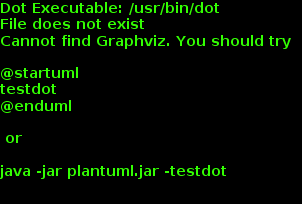
\includegraphics[width=\textwidth,height=\textheight,keepaspectratio]{./images/combat.png}}
	
   \end{section}

   \begin{section}{Bureaucracy - Positive and Negative Attention}
    \textbf{Madeleine Brennan, Elizabeth Hernandez}

    \centerline{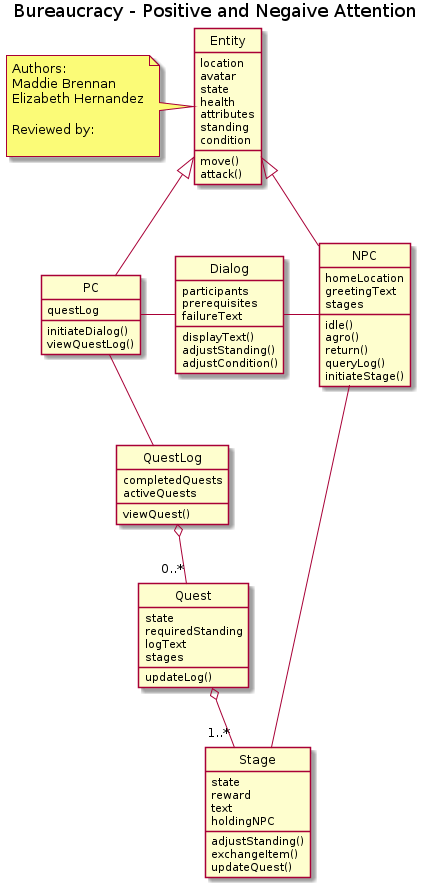
\includegraphics[width=\textwidth,height=\textheight,keepaspectratio]{./images/Class_Diagram.png}}

    \textbf{Description:}

    Bureaucracy deals with interactions between entities in the game, with the biggest interaction within this category being quests. The diagram above visually shows the classes that are related to receiving and completing quests. This relates to bureaucracy because completing quests will help achieve higher approval ratings with the faction that hosts the quest.

    The root class is titled "Entity" and defines basic features of all characters in the game.
    The classes "NPC" and "PC", which stand for "non-player character" and "player character" respectively, are extensions of the Entity class. 
    Each PC will track the state of their quests in a Quest Log. 
    The Quest Log will consist of 0 to many quests.
    Each Quest consists of 1 to many quest Stages.
    Stages hold requirements and rewards for each step of progression in its parent Quest.
    Each Stage is held by an NPC.
    A PC must engage in Dialog with an NPC in order to gain and advance through Stages of their Quests.
\end{section}

\begin{section}{Map and Movement}
    \textbf{Brett Menzies, Gabriel Giovanini de Souze}

    \centerline{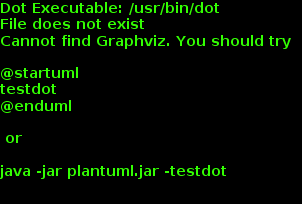
\includegraphics[width=\textwidth,height=\textheight,keepaspectratio]{./images/map_and_movement.png}}
    \textbf{Description:}
    The map subsystem revolves around the\`{ }Map'' class,
    which is composed of a\`{ }Layout'' and a\`{ }Tile set'',
    and aggregates sets of ``Item Position'' and ``Player Position'' classes.
    A\`{ }Renderer'' class requires an instance of a\`{ }Map'';
    Its other connections are outside the scope of this diagram.
    A\`{ }Tile set'' aggregates ``Tiles'' (fixed size map tiles) and 
    ``Sprites'' (Other images drawn on a map, like items and characters) for use by the map and rendering code.
    Each ``Item position'' object represents the position and sprite id of items that have been dropped on the map.
    ``Character position'' acts similarly, except it can be modified by\`{ }input'', which represents 
    networked, npc, and local player inputs for the purposes of this diagram.
  \end{section}
 
  \begin{section}{Player}
     \textbf{Michael Mueller, Alexia Doramus}\\

     \centerline{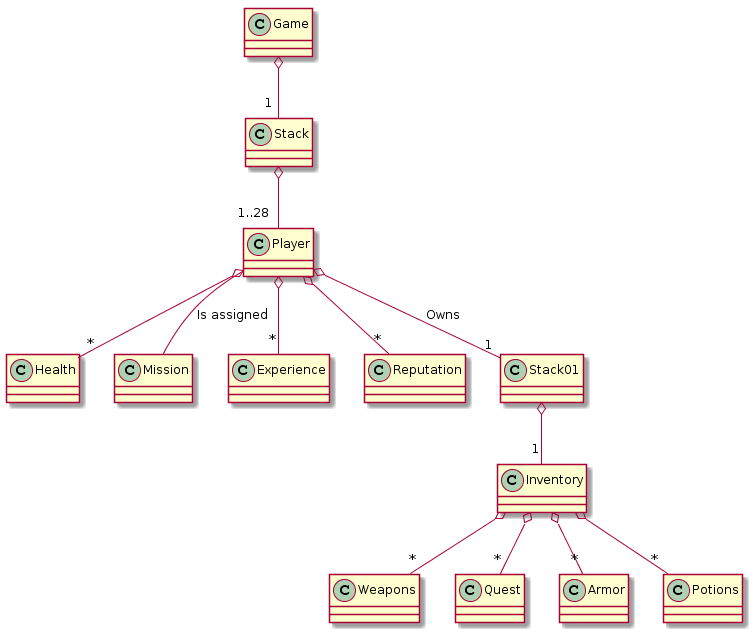
\includegraphics[width=\textwidth]{./images/playerclass.png}}

     \noindent\textbf{Description:}\\
     The player class is an aggregate of multiple parts. It consists of ``health'', ``experience'', ``reputation'', and it owns an ``inventory''. The player class can also be assigned a\`{ }mission''. The\`{ }inventory'' is part of a stack that keeps track of the multiple items, including: ``weapons'', ``quest items'', ``armor'', and ``potions''. The\`{ }player'' is part of a stack which can consist of up to 28 players. The stack that is an aggregation of the players is part of the game.
  \end{section}
  
 \end{chapter}
 \begin{chapter}{Current Project Design: Diagrams}
   \begin{section}{Game State Classes}
   	\centerline{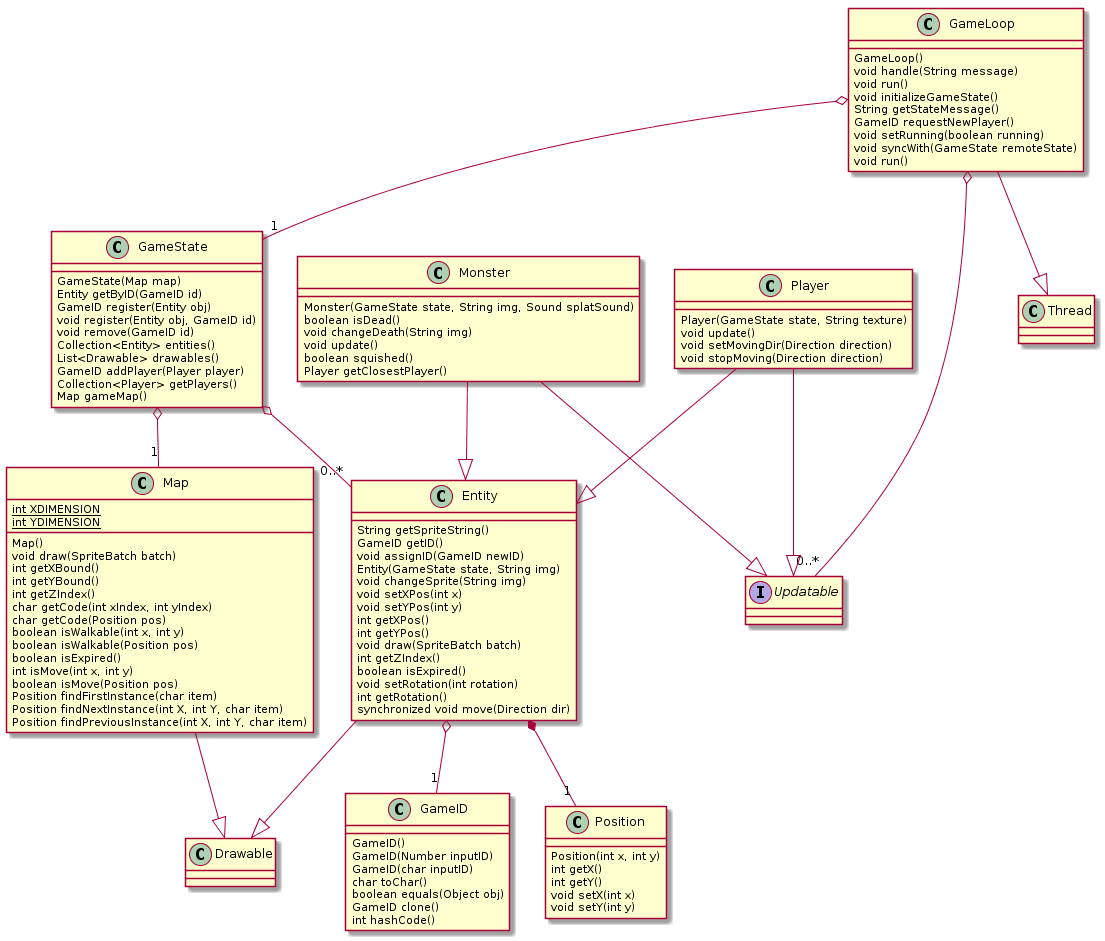
\includegraphics[width=\textwidth,height=\textheight,keepaspectratio]{./images/gameStateClasses.png}}
   \end{section}
   \begin{section}{Input Classes}
   	\centerline{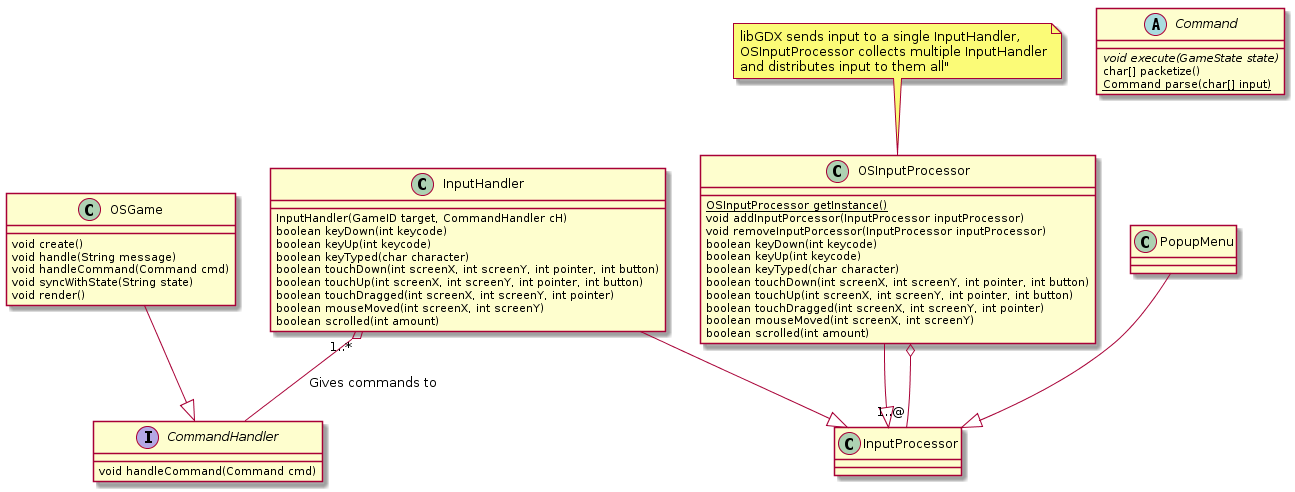
\includegraphics[width=\textwidth,height=\textheight,keepaspectratio]{./images/inputClasses.png}}
   \end{section}
   \begin{section}{Command Classes}
   	\centerline{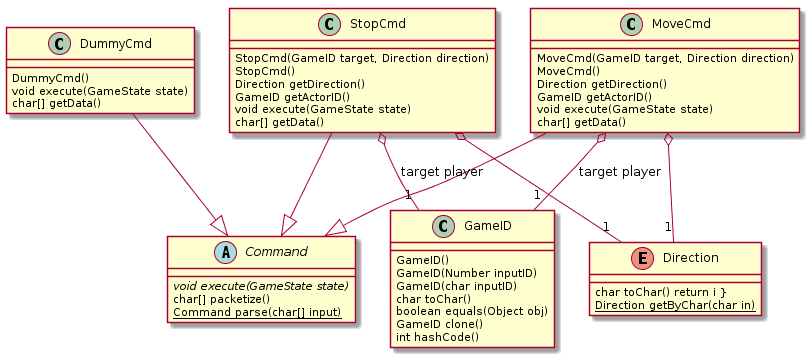
\includegraphics[width=\textwidth,height=\textheight,keepaspectratio]{./images/commandClasses.png}}
   \end{section}
   \begin{section}{Networking Diagrams}
   	\begin{subsection}{Class Diagram}
       	 \centerline{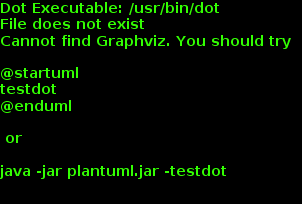
\includegraphics[width=\textwidth,height=\textheight,keepaspectratio]{./images/networkingClasses.png}}
   	\end{subsection}
   	\begin{subsection}{Sequence Diagrams}
   	 \centerline{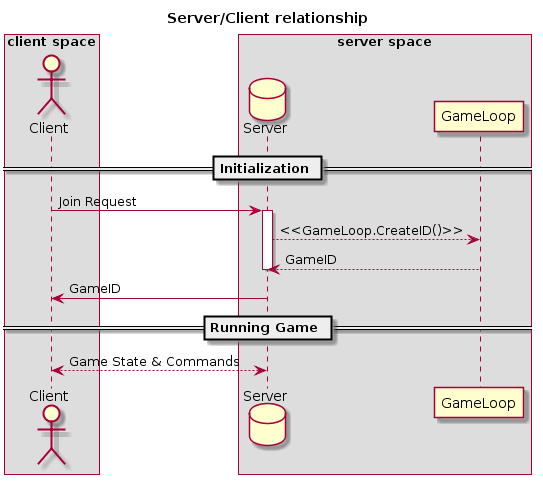
\includegraphics[width=\textwidth,height=\textheight,keepaspectratio]{./images/serverClient.png}}
	\end{subsection}
   \end{section}
 \end{chapter}
 
  \begin{chapter}{Metrics}
  	We chose to use PMD for our software metrics. Specifically, we invoked the Basic, Code Size, Coupling, and Design rulesets. A detailed output is availible as HTML in the ``PMD" folder of our Documentation git repository. In short, PMD's biggest complaints were the high Cyclomatic Complexity of our monster AI (max of 18), a large number of Law of Demeter violations, and some variables that it suggests should be made ``final".
   \begin{section}{Basic}
   \centerline{\includegraphics[width=\textwidth,height=\textheight,keepaspectratio]{./pmdBasic.png}}
   \end{section}
   \begin{section}{Code Size}
      \centerline{\includegraphics[width=\textwidth,height=\textheight,keepaspectratio]{./pmdCodeSize.png}}

   \end{section}
  \end{chapter}
 
 
 \begin{chapter}{jUnit Testing}
 	Our unit testing was run though gradle's test task, which uses JUnit. Our test code is located within the OSGame/core/src/test directory of our project, and run with "gradle test". A "Passed" or "Failed" message will be printed to the terminal for each test run. Standard error and standard output are also piped to the terminal. Gradle automatically makes a parallelized test runner, so there is no "main" to run our tests from.
 	
  \begin{section}{Comms Tests}
   \begin{subsection}{GameID Test}
    \begin{lstlisting}

    public class GameIDTest
    {
    	LwjglApplication lwjglApplication;
    	@Before
    	public void before() throws Exception {
    	}

    @After
    public void after() throws Exception{
    }

    @Test
    public void testGameIDGeneration() throws Exception{
        ArrayList<GameID> seen = new ArrayList<GameID>();
        for (int i=0; i<200; i++) {
            GameID n = new GameID();
            assertTrue(``check previous values'', !seen.contains(n));
            seen.add(n);
        }
    }

    @Test
    public void testCharTranslation() throws Exception{
        GameID origin = new GameID();
        char   idChar = origin.toChar();
        GameID result = new GameID(idChar);
        assertTrue(``Test GameID translation'', result.equals(origin));

        origin = new GameID((Number)42);
        idChar = origin.toChar();
        result = new GameID(idChar);
        assertTrue(``Test GameID translation'', result.equals(origin));
    }


   }

   \end{lstlisting}
  \end{subsection}

  \begin{subsection}{Parser Tester}
   \begin{lstlisting}
   public class ParserTest
   {
    LwjglApplication lwjglApplication;

    public void before() throws Exception
    {
        if (lwjglApplication == null)
        {
            LwjglApplicationConfiguration config = new LwjglApplicationConfiguration();
            config.title = ``Test'';
            config.width = 960;
            config.height = 576;
            lwjglApplication = new LwjglApplication(new ApplicationAdapter()
            {
                @Override
                public void create()
                {
                    super.create();
                }
            }, config);
        }
    }

  /**                                                                                  \
    * Method: Parse(Command[] commands)
    */
    @Test
    public void testParseCommands() throws Exception
    {
        Command[] commands = new Command[3];
        commands[0] = new DummyCmd();
        commands[1] = new DummyCmd();
        commands[2] = new DummyCmd();

        String result = new Parser(new GameState(new Map())).Parse(commands);

        assertEquals(``3,com.comms.DummyCmd:test,com.comms.DummyCmd:test,com.comms.DummyCmd:test,'', result);
    }

   /**
     * Method: DeParseCommands(String data)
     */
    @Test
    public void testDeParseCommands() throws Exception
    {
        String test = ``3,com.comms.DummyCmd:test,com.comms.DummyCmd:test,com.comms.DummyCmd:test,'';

        Command[] result = new Parser(new GameState(new Map())).DeParseCommands(test);

        assertEquals(``com.comms.DummyCmd:test'', new String(result[0].getData()));
        assertEquals(``com.comms.DummyCmd:test'', new String(result[1].getData()));
        assertEquals(``com.comms.DummyCmd:test'', new String(result[2].getData()));
    }

   /**
    * Method: Parse(Entity[] entities)
    */
    @Test
    public void testParseEntities() throws Exception
    {
        String resultString = ``0, ,0,2,2,@,0,2,3,\%,0,2,#,&,0,2,'';                       

        Entity[] entities = new Entity[4];

        Entity entity = new Entity(new GameState(new Map()), ``0'');
        entity.assignID(new GameID(' '));
        entity.setYPos(2);
        entity.setXPos(0);
        entities[0] = entity;

        entity = new Entity(new GameState(new Map()), ``2'');
        entity.assignID(new GameID('@'));
        entity.setYPos(2);
        entity.setXPos(0);
        entities[1] = entity;

        entity = new Entity(new GameState(new Map()), ``3'');
        entity.assignID(new GameID('\%'));                                                 
        entity.setYPos(2);
        entity.setXPos(0);
        entities[2] = entity;

        entity = new Entity(new GameState(new Map()), ``#'');
        entity.assignID(new GameID('&'));
        entity.setYPos(2);
        entity.setXPos(0);
        entities[3] = entity;

        String result = new Parser(new GameState(new Map())).Parse(entities);

        org.junit.Assert.assertEquals(resultString, result);
    }
    
    /**
     * Method: DeParse(String data)                                                      \
     */
        @Test
        public void testDeParse() throws Exception
        { 
        Pair<Entity[],Command[]> pair = new Parser(new GameState(new Map())).DeParse(``4,0, ,0,22,2,@,0,2,3,\%,0,2,#,&,0,2,3,com.comms.DummyCmd:test,com.comms.DummyCmd:test,com.comms.DummyCmd:test,'');
        Entity[] entities = pair.getKey();
        Command[] result = pair.getValue();

        assertEquals(entities[0].getImageCode(), ``0'');
        assertEquals(entities[0].getID().toChar(), ' ');
        assertEquals(entities[0].getYPos(), 22);
        assertEquals(entities[0].getXPos(), 0);

        assertEquals(entities[1].getImageCode(), ``2'');
        assertEquals(entities[1].getID().toChar(), '@');
        assertEquals(entities[1].getYPos(), 2);
	assertEquals(entities[1].getXPos(), 0);

        assertEquals(entities[2].getImageCode(), ``3'');
        assertEquals(entities[2].getID().toChar(), '\%');                                  
        assertEquals(entities[2].getYPos(), 2);
        assertEquals(entities[2].getXPos(), 0);

        assertEquals(entities[3].getImageCode(), ``#'');
        assertEquals(entities[3].getID().toChar(), '&');
        assertEquals(entities[3].getYPos(), 2);
        assertEquals(entities[3].getXPos(), 0);

        assertEquals(``com.comms.DummyCmd:test'', new String(result[0].getData()));
        assertEquals(``com.comms.DummyCmd:test'', new String(result[1].getData()));
        assertEquals(``com.comms.DummyCmd:test'', new String(result[2].getData()));

    }

 \end{lstlisting}
  \end{subsection}

  \begin{subsection}{Command Memento}
   \begin{lstlisting}
    
    @Test
    public void testPacketize() throws Exception {
    GameID testID = new GameID();
    Direction testDir = Direction.NORTH;
    Command orig = new MoveCmd(testID, testDir);

    char[] data = orig.packetize();

    Command result = Command.parse(data);

    assertTrue(``Packetization class test'', result.getClass()==orig.getClass());
    MoveCmd mres = (MoveCmd) result;
    assertTrue(``Direction test'', mres.getDirection().equals(testDir));
    assertTrue(``Actor ID test'' , mres.getActorID().equals(testID));
    }


    \end{lstlisting}
   \end{subsection}
  \end{section}
  \begin{section}{Comms Test Results}
  	test.com.comms.CommandHandlerTest > testAdd PASSED\\
	test.com.comms.CommandHandlerTest > testRemove PASSED\\
	test.com.comms.CommandHandlerTest > testGetInstance PASSED\\
  	test.com.comms.DummyCmdTest > testExecute PASSED\\
  	test.com.comms.DummyCmdTest > testGetData PASSED\\
  	test.com.comms.GameIDTest > testGameIDGeneration PASSED\\
  	test.com.comms.GameIDTest > testCharTranslation PASSED\\
  	test.com.comms.InputHandlerTest > testTouchUp PASSED\\
  	test.com.comms.InputHandlerTest > testKeyDown PASSED\\
  	test.com.comms.InputHandlerTest > testKeyUp PASSED\\
  	test.com.comms.InputHandlerTest > testMouseMoved PASSED\\
  	test.com.comms.InputHandlerTest > testScrolled PASSED\\
  	test.com.comms.InputHandlerTest > testTouchDown PASSED\\
  	test.com.comms.InputHandlerTest > testKeyTyped PASSED\\
  	test.com.comms.InputHandlerTest > testTouchDragged PASSED\\
  	test.com.comms.MoveCmdTest > testExecute PASSED\\
  	test.com.comms.MoveCmdTest > testGetData PASSED\\
  	test.com.comms.MoveCmdTest > testGetDirection PASSED\\
  	test.com.comms.OSInputProcessorTest > testTouchUp PASSED\\
  	test.com.comms.OSInputProcessorTest > testRemoveInputPorcessor PASSED\\
  	test.com.comms.OSInputProcessorTest > testKeyDown PASSED\\
  	test.com.comms.OSInputProcessorTest > testKeyUp PASSED\\
  	test.com.comms.OSInputProcessorTest > testAddInputPorcessor PASSED\\
  	test.com.comms.OSInputProcessorTest > testMouseMoved PASSED\\
  	test.com.comms.OSInputProcessorTest > testScrolled PASSED\\
	test.com.comms.OSInputProcessorTest > testTouchDown PASSED\\
	test.com.comms.OSInputProcessorTest > testKeyTyped PASSED\\
	test.com.comms.OSInputProcessorTest > testTouchDragged PASSED\\
	test.com.comms.OSInputProcessorTest > testGetInstance PASSED\\
	test.com.comms.ParserTest > testParseForEntitiesCommands PASSED\\
	test.com.comms.ParserTest > testParseEntities FAILED\\
    	\hspace{4ex}java.lang.NullPointerException at ParserTest.java:91\\
	test.com.comms.ParserTest > testDePerseEntities FAILED\\
    	\hspace{4ex}java.lang.NullPointerException at ParserTest.java:131\\
	test.com.comms.ParserTest > testDeParseCommands FAILED\\
    	\hspace{4ex}java.lang.NullPointerException at ParserTest.java:74\\
	test.com.comms.ParserTest > testParseCommands FAILED\\
    	\hspace{4ex}java.lang.NullPointerException at ParserTest.java:61\\
	test.com.comms.ParserTest > testDeParse FAILED\\
    	\hspace{4ex}java.lang.NullPointerException at ParserTest.java:167\\
	test.com.comms.StopCmdTest > testExecute PASSED\\
	test.com.comms.StopCmdTest > testGetData PASSED\\
  \end{section}
  
  
  \begin{section}{Renderer Tests}
   \begin{subsection}{Sprite Storage Tests}
    \begin{lstlisting}
    public class SpriteStorageTest
    {

    LwjglApplication lwjglApplication;

    @Before
    public void before() throws Exception
    {
        if(lwjglApplication == null)
        {
            LwjglApplicationConfiguration config = new LwjglApplicationConfiguration();
            config.title = ``Test'';
            config.width = 960;
            config.height = 576;
            lwjglApplication = new LwjglApplication(new ApplicationAdapter()
            {
                @Override
                public void create()
                {
                    super.create();
                }
            }, config);
        }
    }
    
    @After
    public void after() throws Exception
    {
        lwjglApplication.exit();
    }

    /**                                                                                  \
     * Method: getInstance()                                                             \
     */
    @Test
    public void testGetInstance() throws Exception
    {
        assertNotNull(SpriteStorage.getInstance());
    }

    /**                                                                                  \
     * Method: loadAssets()                                                              \
     */
    @Test
    public void testLoadAssets() throws Exception
    {
        try
        {
            SpriteStorage.getInstance().loadAssets();
            assertTrue(``SpriteStorage loaded assets without error'', true);
        } catch (Exception e)
        {
            assertTrue(e.getMessage(), false);
        }
    }

    /**                                                                                  \  
     * Method: getTexture(String code)                                                   \
     */
    @Test
    public void testGetTexture() throws Exception
    {
        assertNotNull(SpriteStorage.getInstance().getTexture(`` ``));                     
        assertNotNull(SpriteStorage.getInstance().getTexture(``X''));
        assertNotNull(SpriteStorage.getInstance().getTexture(``^''));
        assertNotNull(SpriteStorage.getInstance().getTexture(``v''));
        assertNotNull(SpriteStorage.getInstance().getTexture(``@''));
        assertNotNull(SpriteStorage.getInstance().getTexture(``Thomas''));
        assertNotNull(SpriteStorage.getInstance().getTexture(``L''));
        assertNotNull(SpriteStorage.getInstance().getTexture(``D''));
        assertNotNull(SpriteStorage.getInstance().getTexture(``R''));
        assertNotNull(SpriteStorage.getInstance().getTexture(``C''));
        assertNotNull(SpriteStorage.getInstance().getTexture(``M''));
        assertNotNull(SpriteStorage.getInstance().getTexture(``S''));
        assertNotNull(SpriteStorage.getInstance().getTexture(``.''));
        assertNotNull(SpriteStorage.getInstance().getTexture(``|''));
        assertNotNull(SpriteStorage.getInstance().getTexture(``l''));
        assertNotNull(SpriteStorage.getInstance().getTexture(``d''));
        assertNotNull(SpriteStorage.getInstance().getTexture(``r''));
        assertNotNull(SpriteStorage.getInstance().getTexture(``c''));
        assertNotNull(SpriteStorage.getInstance().getTexture(``s''));
        assertNotNull(SpriteStorage.getInstance().getTexture(``T''));
        assertNotNull(SpriteStorage.getInstance().getTexture(``/''));
     }
    }

    \end{lstlisting}
   \end{subsection}
  \end{section}
  \begin{section}{Render Test Results}
  	test.com.renderer.SpriteStorageTest > testLoadAssets FAILED\\
    	\hspace{4ex}com.badlogic.gdx.utils.GdxRuntimeException at SpriteStorageTest.java:37\\
        \hspace{4ex}Caused by: com.badlogic.gdx.utils.GdxRuntimeException at SpriteStorageTest.java:37\\
    	\hspace{4ex}java.lang.NullPointerException at SpriteStorageTest.java:51\\

	test.com.renderer.SpriteStorageTest > testGetTexture FAILED\\
	\hspace{4ex}java.lang.AssertionError at SpriteStorageTest.java:85\\
  \end{section}
 \end{chapter}
\end{document}
